\documentclass[xcolor=pdftex,dvipsnames,table,mathserif,aspectratio=169]{beamer}
\usetheme{metropolis}
%\usetheme{Darmstadt}
%\usepackage{times}
%\usefonttheme{structurebold}

\usepackage[english]{babel}
%\usepackage[table]{xcolor}
\usepackage{pgf,pgfarrows,pgfnodes,pgfautomata,pgfheaps}
\usepackage{amsmath,amssymb,setspace,centernot}
\usepackage[latin1]{inputenc}
\usepackage[T1]{fontenc}
\usepackage{relsize}
\usepackage{pdfpages}
\usepackage[absolute,overlay]{textpos} 

\DeclareMathSizes{10}{10}{6}{6} 


\title [Dynamic Demand I]{Dynamic Demand III:\\
 Hendel Nevo}
\author{C.Conlon}
\institute{Grad IO}
\date{\today}
\setbeamerfont{equation}{size=\tiny}
\begin{document}

\begin{frame}
\titlepage
\end{frame}

\begin{frame}{Today's Readings}
\begin{itemize}
\item Melnikov (Yale PhD Thesis 2001)
\item Gowrisankaran Rysman (JPE)
\item \alert{Hendel and Nevo (Econometrica )}
\item Erdem Imai Keane (2003) also look at a similar problem in Marketing\\
(I am going to skip it this year).
\end{itemize}
\end{frame}


\begin{frame}{Hendel and Nevo (2006)}
\begin{itemize}
\item When a supermarket cuts the price of laundry detergent for a week there is a huge increase in sales.
\item This leads us to conclude consumers are extremely elastic with respect to price
\item When a supermarket makes a permanent price cut to laundry detergent, there is little sales impact in the long run.
\item Now consumers look highly inelastic with respect to price
\item Often we use average prices which include high and low periods in regression studies -- does this make sense?
\item How can we resolve this puzzle?
\end{itemize}
\end{frame}

\begin{frame}{Hendel and Nevo (2006)}
\begin{itemize}
\item Hendel and Nevo suggest that consumers respond by temporary price  reductions by stockpiling inventories.
\item Consumers spend down their inventories during periods of high prices
\item Consumers have variable storage costs and price sensitivities. Why?
\item This has implications for inter temporal price discrimination and retail High-Low pricing strategies.
\end{itemize}
\end{frame}

\begin{frame}{Data}
\begin{itemize}
\item 9 Supermarkets in a large midwest city (Dominick's in Chicago)
\item Store-level: for each brand 13 ($j$) size $x$: 32-256oz in each store, each week ($t$)
\begin{enumerate}
\item Price $p_{jxt}$ 
\item Quantity $q_{jxt}$
\item Promotions $a_{jxt}$ (binary for feature/display)
\end{enumerate}
\item Consumers are of type $h$ with utility: $u(c_{ht} + \nu_{ht}; \theta_h)$
\item Current consumption is $c_{ht} = \sum_j c_{jht}$ \alert{not brand specific!}
\item There is a shock affected marginal utility of consumption $\nu_{ht}$.
\item Decision: $d_{hjxt} = 1$ is a purchase of $h$ of brand $j$ and size $x$ at $t$. (includes outside option $=0$).
\end{itemize}
\end{frame}

\begin{frame}{Table 3: Sales}
\begin{figure}[htbp]
\begin{center}
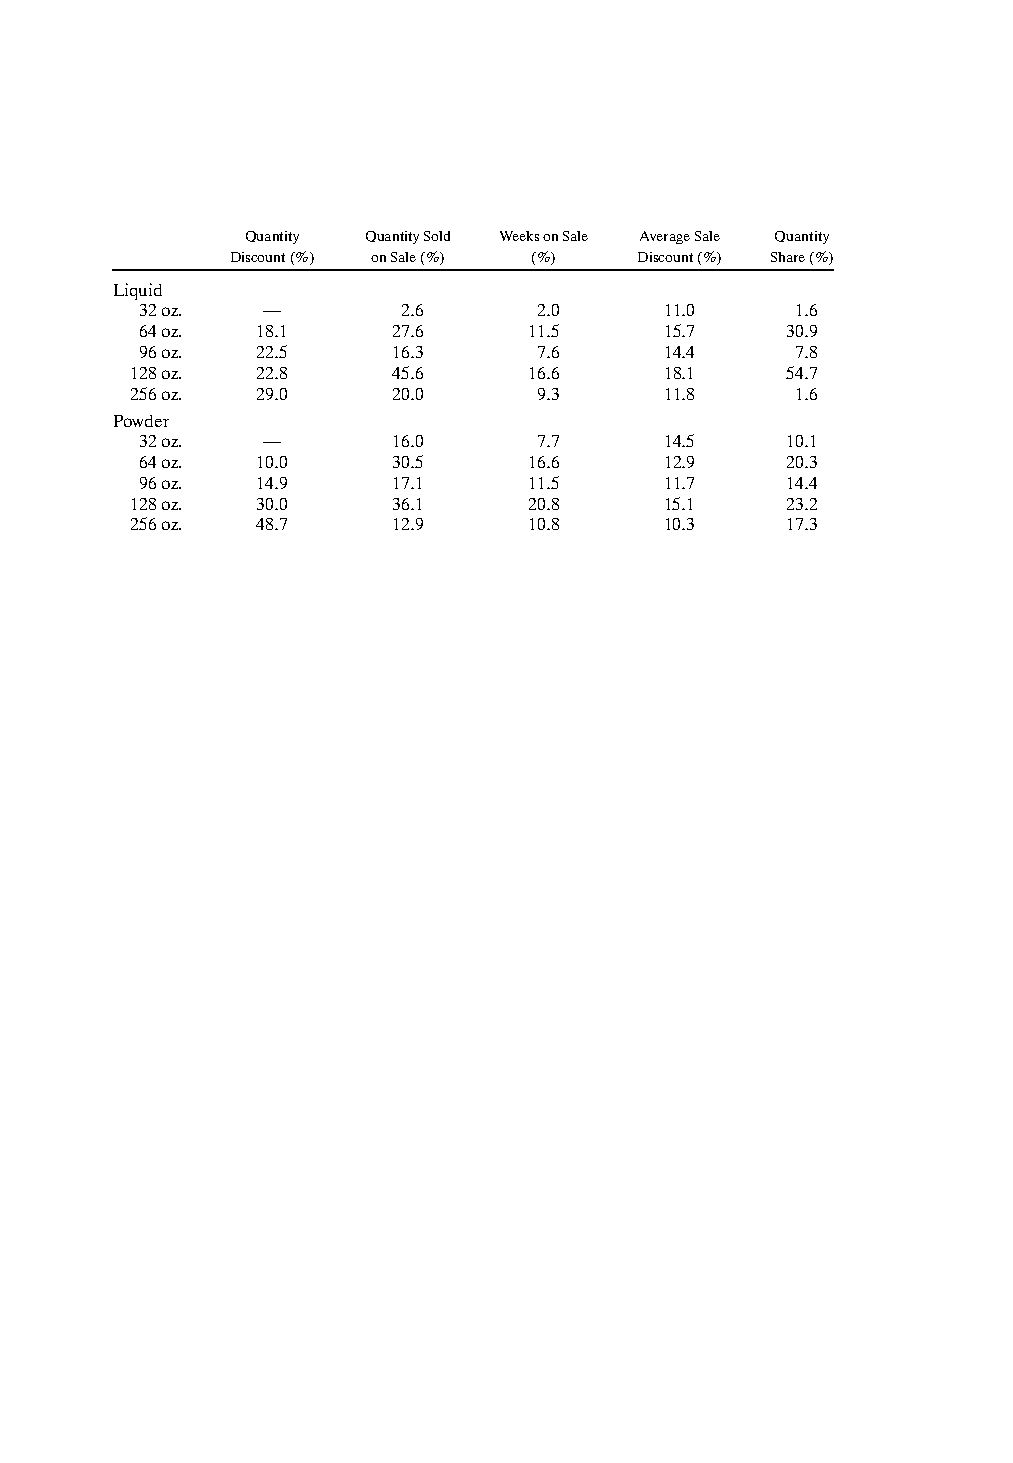
\includegraphics[width=4in]{resources/hntable3.pdf}
\label{gandr1}
\end{center}
\end{figure}
\end{frame}


\begin{frame}{Dynamic Discrete Choice}
\footnotesize
\begin{eqnarray*}
V(s_t)&=& \max_{c_h(s_t),d_{jxt}(s_t)} \sum_t \beta^{t-1} E[ u(c_{ht}+\nu_{ht}; \theta_h) - C_h(i_{h,t+1};\theta_h) \\
&+&\sum_j d_{hjxt} (\alpha_h^p p_{jxt} + \xi_{hjx} + \alpha_h^a a_{jxt} + \epsilon_{hjxt} )| s_t]\\
i_{h,t+1} &=& i_{ht} + x_{ht} - c_{ht}\\
\sum_{j,x} d_{hjxt} &=& 1
\end{eqnarray*}
\begin{itemize}
\item Abuse of notation: $x_{ht}$ is size of the choice
\item $C_h(i; \theta_h)$ is cost of storage
\item $s_t$ contains current inventory $i_t$, current prices, and consumption shock $\nu_t$ as well as $\epsilon_{ht}$.
\item $\xi_{jhxt}$ captures expected future differences in utility of $x$ units of $j$ at time of purchase.
\begin{enumerate}
\item as long as discounting is low
\item brand-specific differences in utility (but not consumption) enter linearly.
\end{enumerate}
\end{itemize}
\end{frame}

\begin{frame}{Model Assumptions}
\begin{block}{Assumption 1}
$\nu_t$ is independently distributed over time and across consumers.\\
 \alert{No serial correlation!}
\end{block}
\begin{block}{Assumption 2}
Prices $p_{jxt}$ and advertising $a_{jxt}$ follow an exogenous first-order Markov process.\\
\alert{Hard to justify this with a model of profit maximizing supply!}
\end{block}
\begin{block}{Assumption 3}
$\epsilon_{jxt}$ is i.i.d. extreme value type 1.
\end{block}
\end{frame}

\begin{frame}{Likelihood}
Conditional on Household we can write the probability of a sequence of purchase decisions:
\begin{eqnarray*}
P(d_1,\ldots,d_t | p_1,\ldots,p_T) = \int \prod_t P(d_t | p_t, \\
i_t(d_{t-1},\ldots,d_1, \nu_{t-1},\ldots,\nu_1,i_1))dF(\nu_1,\ldots,\nu_T) dF(i_1)
\end{eqnarray*}
\begin{itemize}
\item Beginning of period inventory depends on previous decisions, previous shocks, and initial inventory.
\item $p_t$ now includes all observed state variables not just prices
\end{itemize}
\end{frame}

\begin{frame}{Choice Problem}
\begin{eqnarray*}
Pr(d_{jx} | p_t,i_t,\nu_t) &=& \frac{\exp[\alpha p_{jxt} + \xi_{jx} + \beta a_{jxt} + M(s_t,j,x)]}{\sum_{k,y} \exp[\alpha p_{kyt} + \xi_{jy} + \beta a_{kyt} + M(s_t,k,y)]}\\
M (s_t,j,x) &=& \max_c [ u(c+\nu_t) - C(i_{t+1}) + \beta E[V(s_{t+1}|d_{jx},c,s_t]]\\
\end{eqnarray*}
\begin{itemize}
\item State space has very high dimension. (Lots of brand-size combos at different prices)
\item Keeping track of all brands/prices would be very costly
\end{itemize}
\end{frame}

\begin{frame}{3-step Procedure}
To reduce complexity, Hendel and Nevo propose a 3-step estimator
\begin{itemize}
\item Maximize likelihood of observed brand choice \alert{conditional} on size in order to recover the $(\alpha,\xi)$ parameters.
\item This avoids solving MDP but instead is just static discrete choice problem (efficiency loss!)
\item Second step: compute \alert{inclusive values} for each size and transition probability matrix.
\item Now solve a quantity choice only nested fixed point problem. The key is that there is \alert{only one ``index price'' per size}.
\item The reason this is feasible is our old friend, the \alert{conditional independence assumption} (of what?)
\end{itemize}
\end{frame}

\begin{frame}{Step 1: Brand Choice}
\begin{eqnarray*}
Pr(d_{jx} | x_t, p_t,i_t,\nu_t) &=& \frac{\exp[\alpha^p p_{jxt} + \xi_{jx} + \alpha^a a_{jxt}]}{\sum_{k,y} \exp[\alpha^p p_{kyt} + \xi_{jy} + \alpha^a a_{kyt}  ] }\\
&=&Pr(d_{jx} | x_t, p_t)
\end{eqnarray*}
\begin{itemize}
\item The trick is that $M(s_t,j,x)$ is the same for all products of the same size $x$.
\item This means the dynamics drop out of the brand-choice equation conditional on $x_t$.
\item We can recover $(\alpha, \xi)$ from static demand estimation!
\end{itemize}
\end{frame}

\begin{frame}{Step 2: Inclusive Values}
\begin{eqnarray*}
\omega_{xt} &=& \log \left( \sum_k \exp(\alpha^p p_{kxt} + \xi_{xt} + \alpha^a a_{kxt}) \right)
\end{eqnarray*}
\vspace{-0.5cm}
\begin{block}{Assumption 4: IVS}
$$F(\omega_t | s_{t-1}) = F(\omega_t | \omega_{t-1})$$
\end{block}
\begin{itemize}
\item Compute ex-ante expected utility of purchasing size $x$ in period $t$
\item Does not depend on which $j$ is purchased.
\item IVS means we can keep track of a lot less information!
\item Same as G\&R two price vectors with same inclusive values must have same transition probabilities.
\item Do individual prices still matter? (Test)
\end{itemize}
\end{frame}


\begin{frame}{Step 3: Dynamic Choice of Size}
\begin{eqnarray*}
V(i,\omega_t,\epsilon_t,\nu_t) = \max_{c,x} [ u(c + \nu_t) - C(i_{t+1}) + \omega_{xt} + \epsilon_{xt} + \\
\beta E[V(i_{t+1},\omega_{t+1},\epsilon_{t+1},\nu_{t+1}) | i_t, \omega_t, \epsilon_t, \nu_t, c, x] ]
\end{eqnarray*}

\begin{itemize}
\item Compute ex-ante expected utility of purchasing size $x$ in period $t$
\item Does not depend on which $j$ is purchased.
\item IVS means we can keep track of a lot less information!
\item Same as G\&R two price vectors with same inclusive values must have same transition probabilities.
\item Do individual prices still matter? (Test)
\end{itemize}
\end{frame}

\begin{frame}{Key Proposition}
How do we know that the simplified problem has the same solution as the original dynamic problem?
\begin{eqnarray*}
P(x_t | i_t,p_t, \nu_t) = P(x_t | i_t, \omega(p_t),\nu_t)
\end{eqnarray*}

\begin{itemize}
\item Before we got to see the entire state $s_t$
\item Now we only see the expected utility of $x_t$ aka $\omega_{xt}$
\item The proof relies on Assumption 3(IID Logit errors) and Assumption 4 (IVS).
\end{itemize}
\end{frame}

\begin{frame}{Computational Details}
Iterate policy evaluation and policy improvement 
\begin{enumerate}
\item Approximate the value function by a polynomial function of $s_t$. (Logarithmic)
\item Guess an optimal policy and minimized (LSQ) deviation between the value function and expected future value
\item Update the policy function for every state
\item Update expectation with coefficients and expected value of state variables
\item Repeat until value function coefficients converge
\end{enumerate}
This is a \alert{Smooth Approximation} approach
\end{frame}


\begin{frame}{Table 4: Brand Choice Estimates}
\begin{figure}[htbp]
\begin{center}
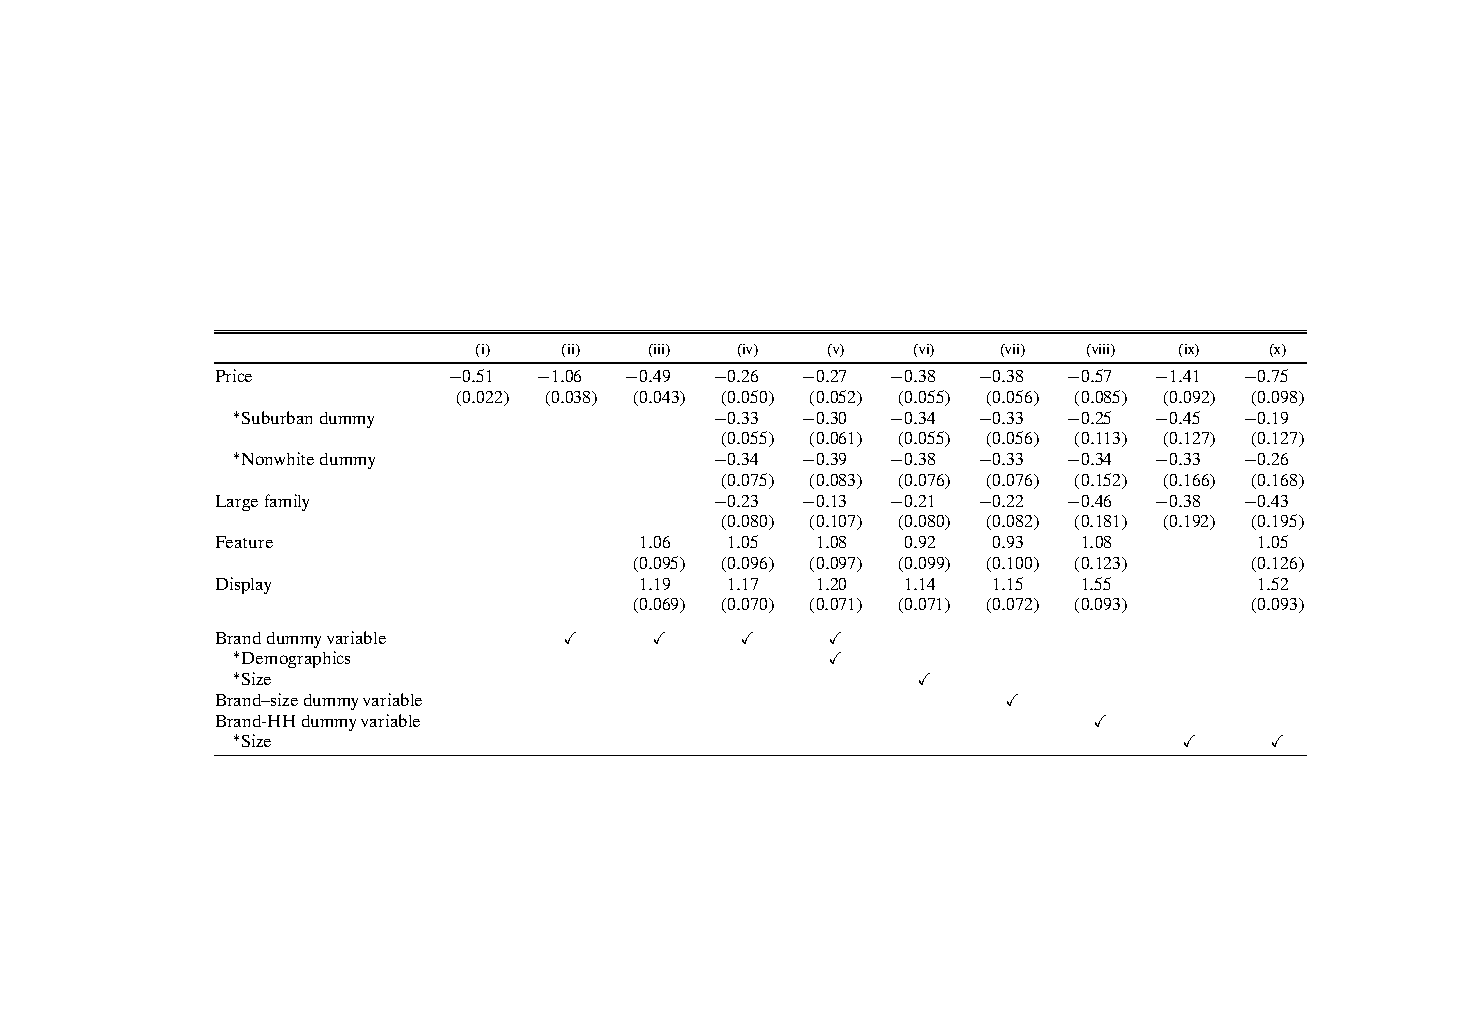
\includegraphics[width=4in]{resources/hntable4.pdf}
\label{gandr1}
\end{center}
\end{figure}
\end{frame}

\begin{frame}{Table 5: Belief Process Estimates}
\begin{figure}[htbp]
\begin{center}
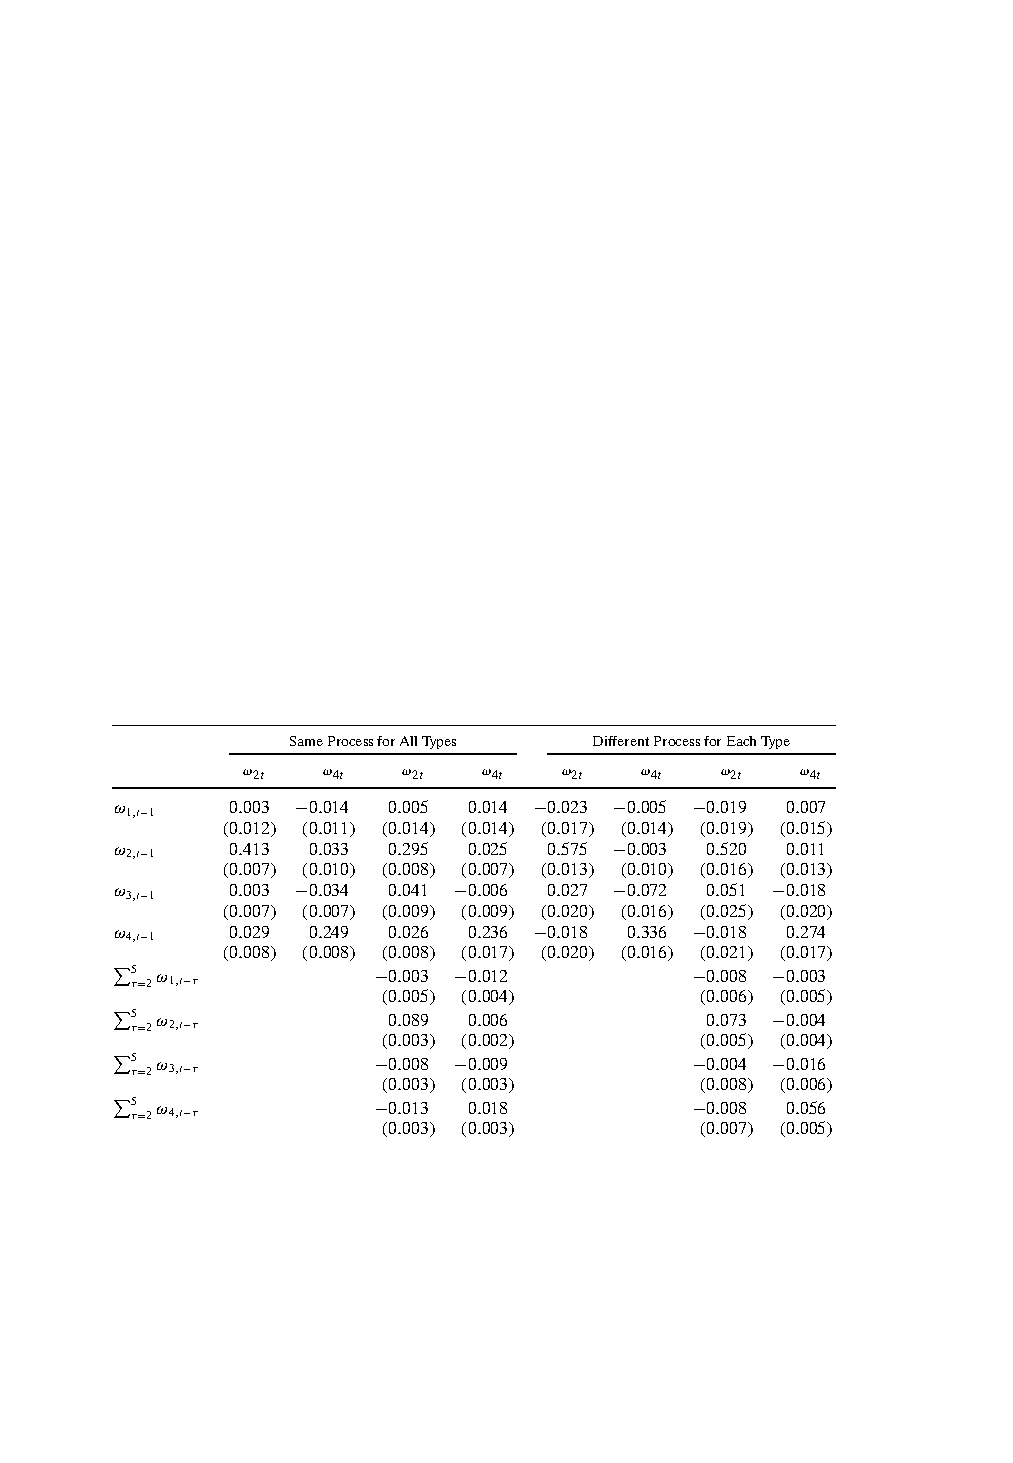
\includegraphics[width=4in]{resources/hntable5.pdf}
\label{gandr1}
\end{center}
\end{figure}
\end{frame}

\begin{frame}{Table 5: Dynamic Problem Estimates}
\begin{figure}[htbp]
\begin{center}
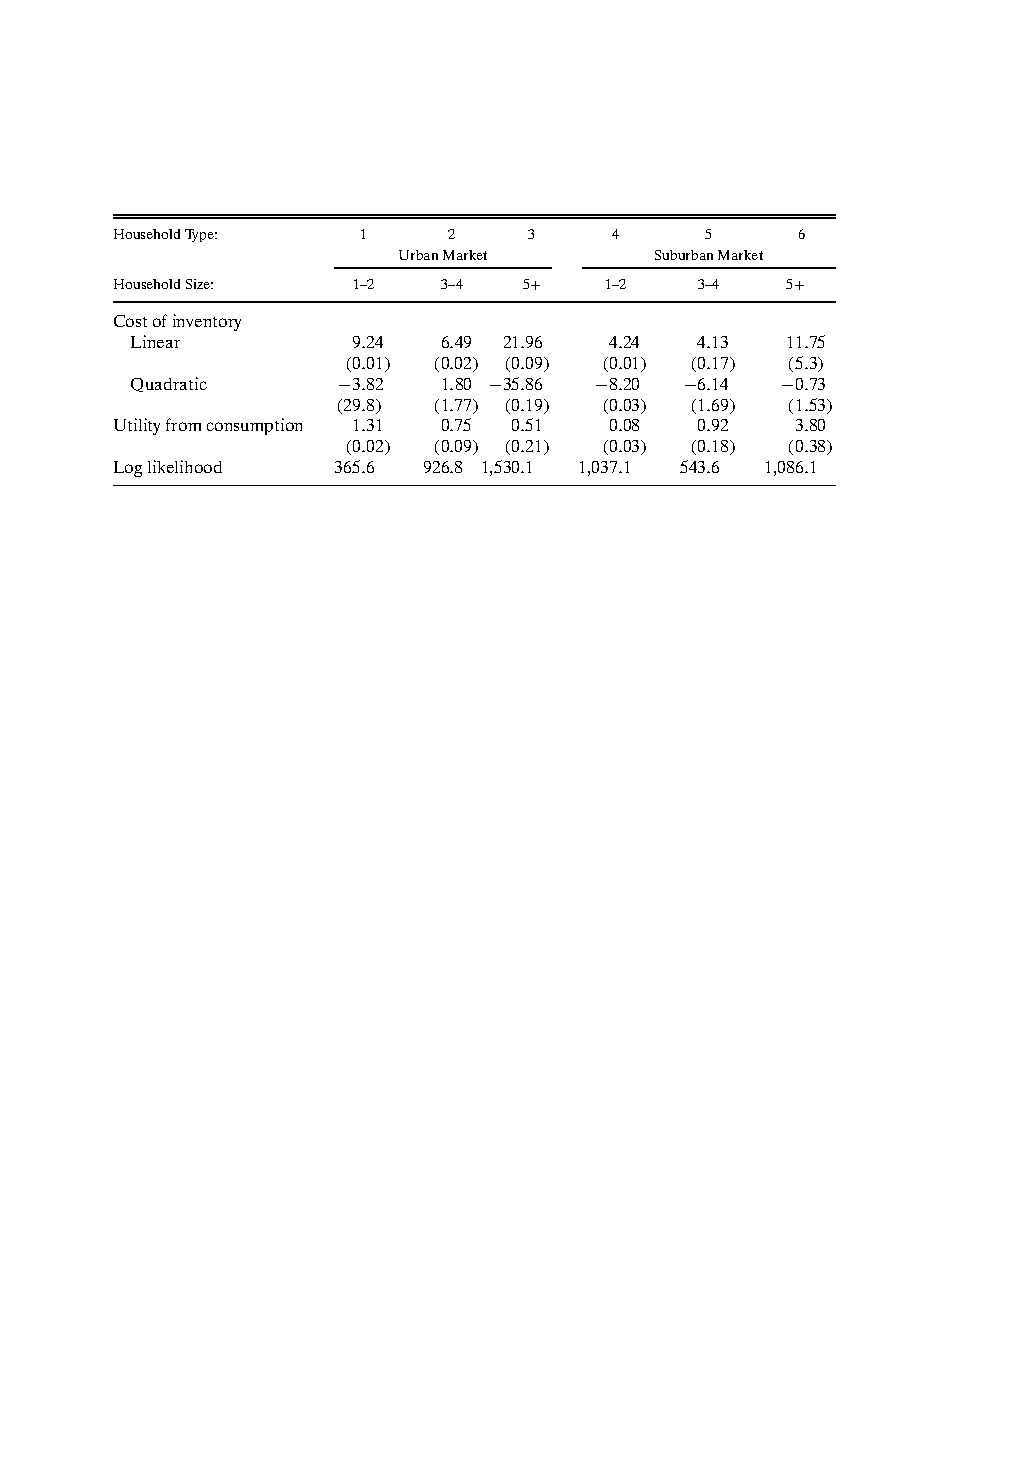
\includegraphics[width=4in]{resources/hntable6.pdf}
\label{gandr1}
\end{center}
\end{figure}
\end{frame}

\begin{frame}{Table 8: Elasticities Compared to Static Model}
\begin{figure}[htbp]
\begin{center}
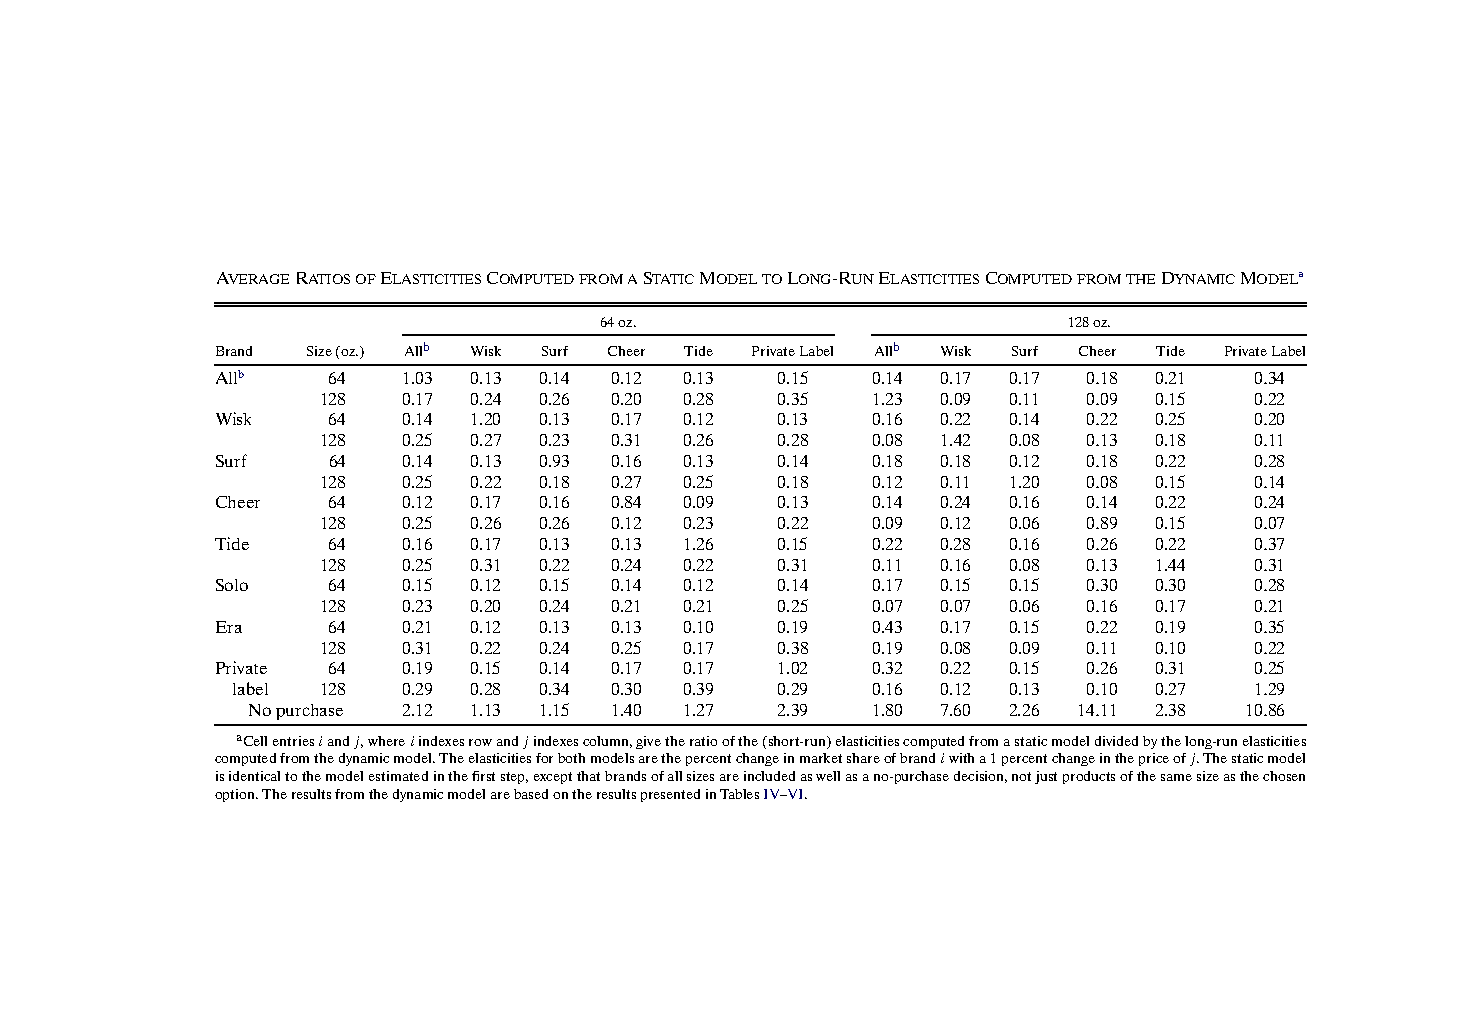
\includegraphics[width=4in]{resources/hntable8.pdf}
\label{gandr1}
\end{center}
\end{figure}
\end{frame}
\end{document}